\hypertarget{SWE__Block_8cpp}{}\section{app/src/main/cpp/blocks/\+S\+W\+E\+\_\+\+Block.cpp File Reference}
\label{SWE__Block_8cpp}\index{app/src/main/cpp/blocks/\+S\+W\+E\+\_\+\+Block.\+cpp@{app/src/main/cpp/blocks/\+S\+W\+E\+\_\+\+Block.\+cpp}}
{\ttfamily \#include \char`\"{}S\+W\+E\+\_\+\+Block.\+hh\char`\"{}}\\*
{\ttfamily \#include \char`\"{}../tools/help.\+hh\char`\"{}}\\*
{\ttfamily \#include $<$cmath$>$}\\*
{\ttfamily \#include $<$iostream$>$}\\*
{\ttfamily \#include $<$cassert$>$}\\*
{\ttfamily \#include $<$limits$>$}\\*
Include dependency graph for S\+W\+E\+\_\+\+Block.\+cpp\+:\nopagebreak
\begin{figure}[H]
\begin{center}
\leavevmode
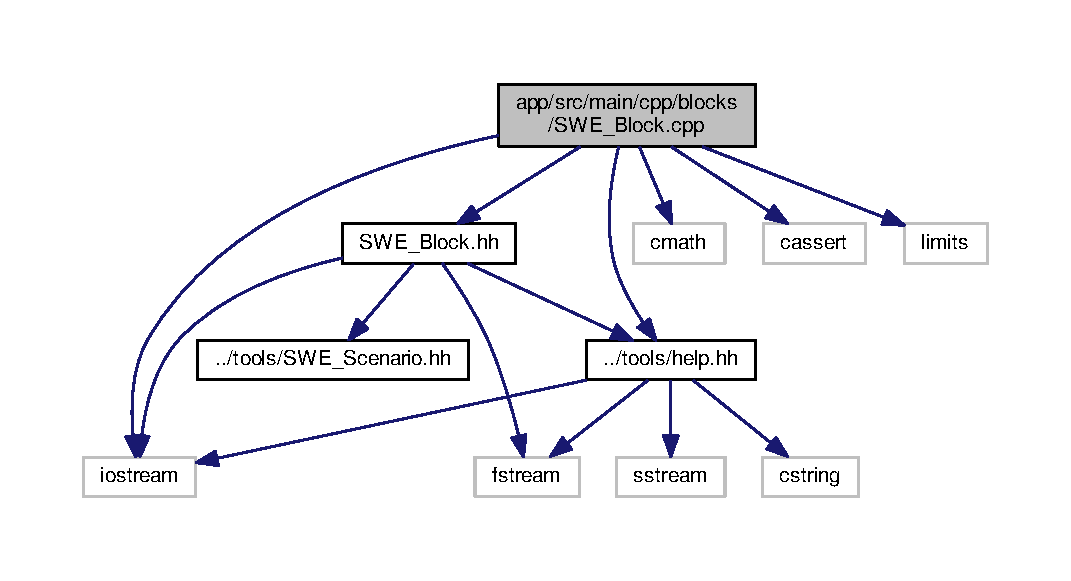
\includegraphics[width=350pt]{SWE__Block_8cpp__incl}
\end{center}
\end{figure}


\subsection{Detailed Description}
This file is part of S\+WE.

\begin{DoxyAuthor}{Author}
Michael Bader, Kaveh Rahnema, Tobias Schnabel 

Sebastian Rettenberger (rettenbs AT in.\+tum.\+de, \href{http://www5.in.tum.de/wiki/index.php/Sebastian_Rettenberger,_M.Sc}{\tt http\+://www5.\+in.\+tum.\+de/wiki/index.\+php/\+Sebastian\+\_\+\+Rettenberger,\+\_\+\+M.\+Sc}.)
\end{DoxyAuthor}
\hypertarget{help_8hh_LICENSE}{}\subsection{L\+I\+C\+E\+N\+SE}\label{help_8hh_LICENSE}
S\+WE is free software\+: you can redistribute it and/or modify it under the terms of the G\+NU General Public License as published by the Free Software Foundation, either version 3 of the License, or (at your option) any later version.

S\+WE is distributed in the hope that it will be useful, but W\+I\+T\+H\+O\+UT A\+NY W\+A\+R\+R\+A\+N\+TY; without even the implied warranty of M\+E\+R\+C\+H\+A\+N\+T\+A\+B\+I\+L\+I\+TY or F\+I\+T\+N\+E\+SS F\+OR A P\+A\+R\+T\+I\+C\+U\+L\+AR P\+U\+R\+P\+O\+SE. See the G\+NU General Public License for more details.

You should have received a copy of the G\+NU General Public License along with S\+WE. If not, see \href{http://www.gnu.org/licenses/}{\tt http\+://www.\+gnu.\+org/licenses/}.\hypertarget{help_8hh_DESCRIPTION}{}\subsection{D\+E\+S\+C\+R\+I\+P\+T\+I\+ON}\label{help_8hh_DESCRIPTION}
T\+O\+DO 